\documentclass[11pt]{article}
\usepackage[margin =1in]{geometry}
\usepackage{authblk}
\usepackage{multicol}
\usepackage{graphicx}
\usepackage{subcaption}
\usepackage{float}
\usepackage[hidelinks]{hyperref}
\usepackage{csquotes}
\MakeOuterQuote{"}
\usepackage{amsmath}
\usepackage[backend = bibtex, style = numeric, sorting = ynt]{biblatex}
\addbibresource{reference.bib}
\title{{\bf Comparing Computational Methods for RNA Secondary Structure Prediction}}
\author[1]{Harrison LaBollita}
\author[2]{Petr \u Sulc}
\date{}
\affil[1]{Department of Physics, Arizona State University, Tempe, AZ 85281 USA}
\affil[2]{Center for Biological Physics, Arizona State University, Tempe, AZ 85281 USA}

\begin{document}

\maketitle
\begin{abstract}
Text goes here.
\end{abstract}
\tableofcontents
\section{Introduction}


\begin{multicols}{2}
\section{Datasets}
We used two independent datasets to benchmark the performance of our CNN and Gillespie algorithm, respectivley. The dataset we used to train, validate and test our CNN contained over 50,000 RNA sequences all of the length 30 nucleotides (ntds). This dataset was generated using NUPACK software \cite{doi:10.1002/jcc.21596}. While it is desirable for CNN to function with variable length sequences, to benchmark performance of our model it was sufficient to use homogenous length sequences.


For our CNN model, we must encode the sequence and dotbracket information in such a way for the computer to understand it. The sequences are transformed into a matrix, which is described in more detail in a later section. The dotbracket representation is also transformed into a $N \times 3$ matrix, where $N$ is the number of ntds in the sequence and the three columns represent '(', ')', or '.'. A $1$ is placed in the appropriate represenation and $0$'s are placed in the remaining columns. For example, if the dot bracket representation of the secondary structure was '((..))', then we would encode this information in the following matrix:


\begin{center}
{\bf ((..))}\\

\begin{tabular}{|c|c|c|}
\hline
1 & 0 & 0\\
1 & 0 & 0\\
0 & 0 & 1\\
0 & 0 & 1\\
0 & 1 & 0\\
0 & 1 & 0\\
\end{tabular}
\end{center}

We created a second dataset from the \href{https://rfam.xfam.org}{Rfam database}, which is an online colletion of thousands of RNA families that contain the sequence, secondary structure, and the free energy of the secondary structure \cite{ 10.1093/nar/gkv480, doi:10.1002/cpbi.51}. This dataset contains 27 sequences with variable lengths. The complete dataset statistics are contained in Figure \ref{fig:rfam}. In a later section, we benchmark the performance of our stem level gillespie algorithm compared to a leading secondary structure predictor, Vienna RNA \cite{Lorenz2011}.

\begin{figure}[H]
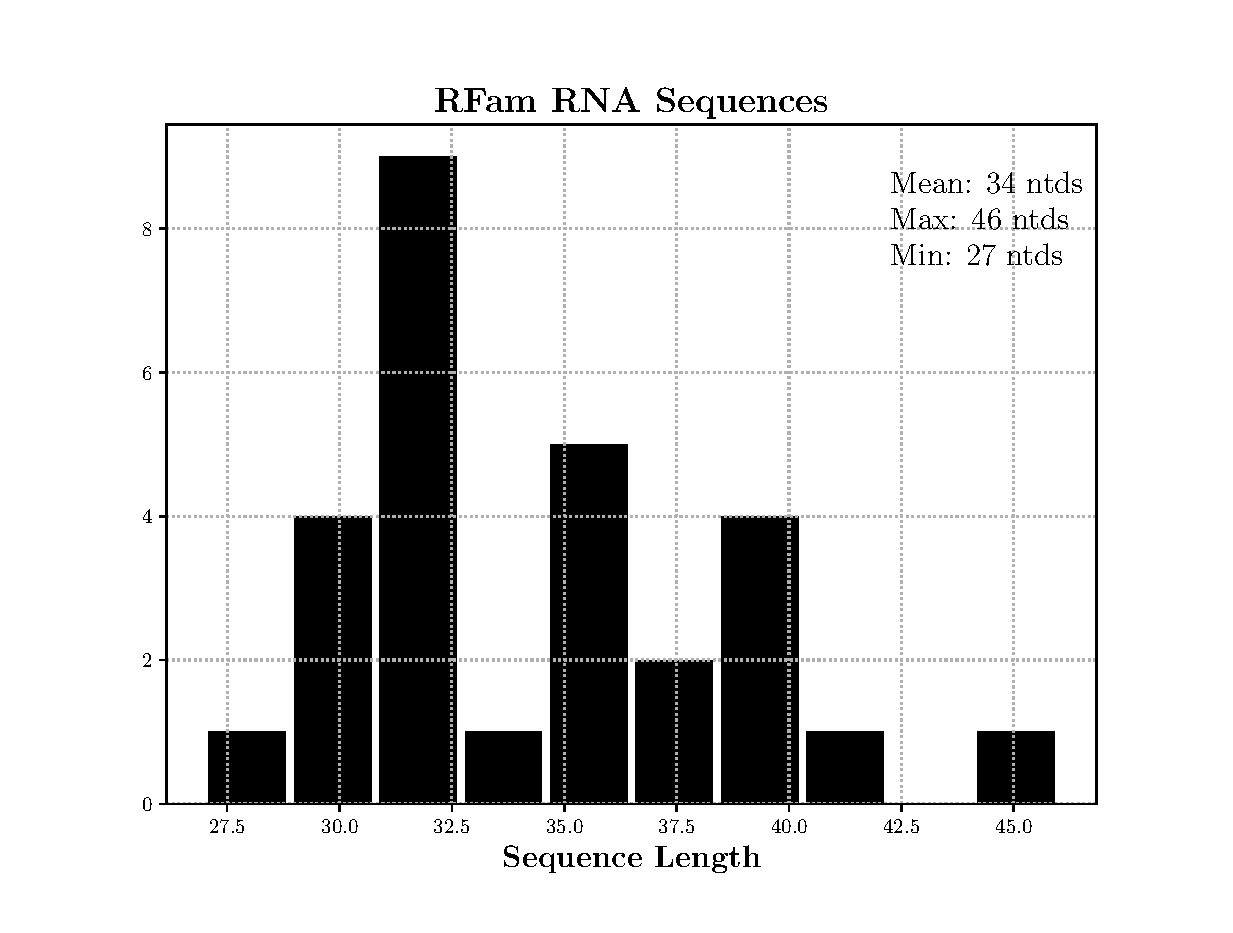
\includegraphics[width = 0.6\textwidth]{fig/rfam}
\caption{The Rfam dataset contains 27 total sequences with variable length. The average length is 34 ntds. The longest sequences is 46 ntds and the shortest sequence is 27 ntds.}
\label{fig:rfam}
\end{figure}
\end{multicols}

\begin{multicols}{2}
\section{CNN Predicts Secondary Structure}
Convolutional neural networks (CNN)s are machine learning algorithms that are primarily used for image classification problems. The input layer is the image’s RGB values, which are then fed through multiple convolution layers, that are finally connected to a standard fully-connected feed forward neural network. Ultimately, to use a CNN one must have data that can be interrupted as an image. Following \cite{10.3389/fgene.2019.00467}, we have replicated their CNN in PyTorch \cite{paszke2017automatic} in efforts to achieve similar results.


\subsection{Matrix Representation of RNA}

RNA sequences are comprised of any combination of four nucleotide bases: adenine (A), guanine (G), cytosine (C), and uracil (U). When using ML techniques for RNA secondary structure prediction, a formidable challenge is how to encode the sequence as input for the ML architecture. We have chosen to encode the sequence as a matrix in order to use a CNN architecture. The rules of folding a RNA secondary structure are very simple: A pairs with U, G pairs with C, and sometimes G pairs with C. The canonical pairs A-U and G-C are called Watson-Crick pairs (CITE), while the G-U pair is known as the wobble pair. Following these simple rules, we can build a weighted matrix based on which base is more likely to pair with whom. The complete matrix building algorithm is explain in \cite{10.3389/fgene.2019.00467}, and our source code is available on this \href{https://github.com/harrisonlabollita/RNA-ML/blob/master/src/explore/cnn%20code/rna2matrix.py}{GitHub repository}.

\subsection{Model}

The architecture of our CNN is simple. The  model contains two convolutional layers, two pooling layers, and three fully-connected layers. We use a binary cross-entropy loss function, since we are predicting either a value of 0 or 1. We optimized the hyperparameters in our model via configuration space searching, where we randomly choose parameters from our configuration space, train our network and log the performance. We found that a learning rate of 0.001 and momentum of 0.9 performed the best without overfitting.

We have illustrated the workflow of our CNN Model in Figure \ref{fig:cnn_model}. We begin with an RNA sequence, convert the sequence into a matrix, then feed it into our CNN. The output of the CNN is a $N \times 3$ matrix, where $N$ is the number of nucleotides in the sequence and our model's predicted values of each nucleotide being paired or unpaired. From this information, we reconstuct the dotbracket representation by choosing the highest value in each row as the model's choice for paired ("(" or ")") or unpaired (".") and compare our predicted structure with the actual secondary structure for this sequence.
\end{multicols}

\begin{figure}[H]
\centering
\hspace*{-8cm}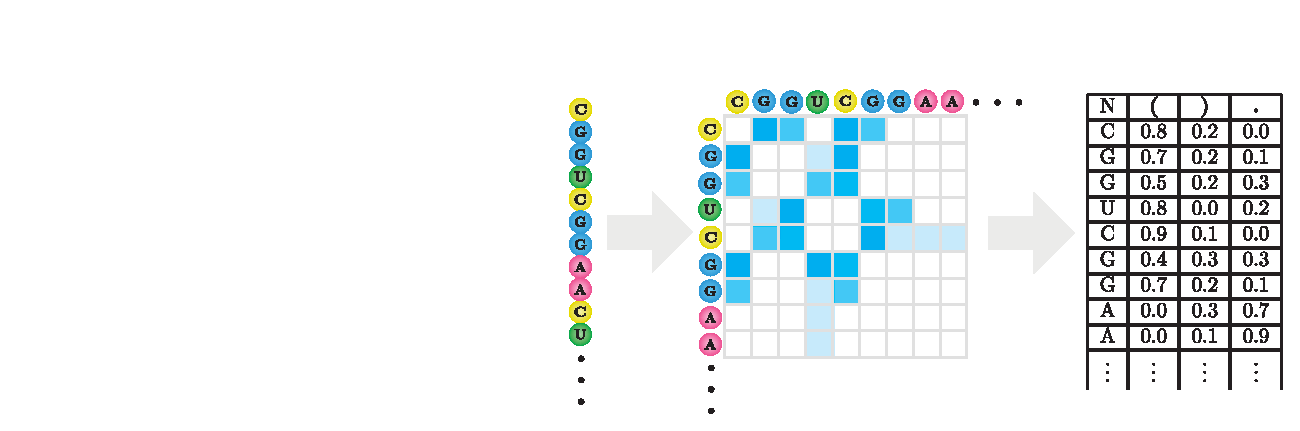
\includegraphics{fig/cnn_model_outline}
\caption{We convert our dataset of RNA sequences into a new dataset of RNA matrices. These matrices are used as inputs into our CNN. Notice that the darker blue squares correspond to heavier weighted base meaning more likely to be paired. The output of our network is the matrix on the far right which we use to reconstruct the dot bracket represenation of the secondary structure.}
\label{fig:cnn_model}
\end{figure}

\begin{multicols}{2}
We trained and validated our CNN model on dataset containing 50,000 uniform length RNA sequences following the standard condition, where 80\% of the data is used for training and 20\% of the dataset was used for validation. We trained our network for 100 epochs with a batchsize of 100. We quantified the accuracy of our model by counting the number of mistakes our model made when predicting the secondary structure. A perfect prediction corresponds to 0 mistakes.
\end{multicols}

\begin{multicols}{2}
\subsection{Results and Discussion}
In this section, we present our CNN model's performance on RNA secondary structure prediction. In Figure \ref{fig:acc}, we have plotted the training and validation accuracy of our model throughout the training session. We can see that the model converges to about 84\% accuracy for both training and validation accuracies.

Our CNN model achieves similar results to the \cite{10.3389/fgene.2019.00467}, however, our model will sometimes predict non-physical structures. Therefore, it is necessary that we include a dynamic layer in our model that corrects for these non-physical outputs. This is the central weakness of all non-physical secondary structure predictors. Without including knowledge of physical considerations these models will always produce unphysical secondary structures.

\end{multicols}
\begin{figure}[H]
\centering
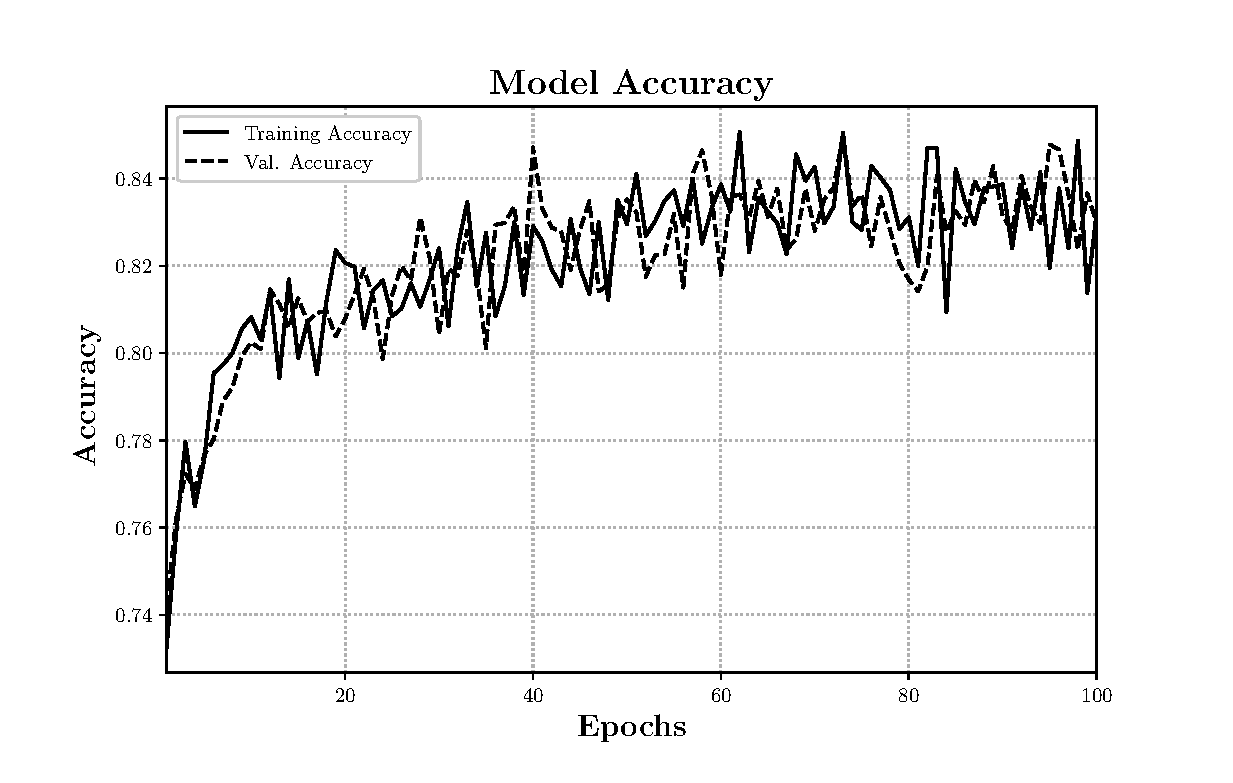
\includegraphics[width = \textwidth]{fig/acc}
\caption{Training and validation accuracy over the 100 epochs. The solid black line is the training accuracy and the dotted black line is the validation accuracy.}
\label{fig:acc}
\end{figure}


\begin{multicols}{2}
\section{Stem Level Gillespie Algorithm}

\subsection{Stem Level Implementation}
There are two central approaches when writing a computer program to simulate RNA folding kinetics: base pairs or stems. The first approach considers the transitions from RNA states at the base pair level, which generates a microscopic picture of the RNA folding events \cite{10.1093/nar/gkv480}. The alternative approach is to consider large arrangements of base pairs or stems. The transition between RNA states is then completed via forming or breaking a complete stem rather than single base pairs. In this work, we propose a gillespie algorithm that works at the stem level. We intend for the algorithm to be used for long RNA stands ($>$ 100+ ntds), therefore, the stem level implementation is computationally more desirable than working at the base pair level.

As mentioned above we implement a gillespie algorithm, which is a stochastic simulation alogrithm to perform our RNA folding kinetics. The gillespie algorithm is very popular for simulating chemical reactions.  For a more complete discussion of the gillespie algorithm please see Ref. \cite{erban2007practical}. We will briefly go over our algorithm and additionally, we have provided an illustration of our algorithm in Figure \ref{fig:gill_algo}.

Our algorithm begins by first defining a set of moves and a set of transition rates that correspond to each move. There are two different rates: one for creating a stem, which we calculate from the entropy

\begin{equation}
\text{Rate of forming stem} = \exp \Big (\frac{ \Delta S}{k_{B}} \Big ),
\end{equation}
where $k_{B}$ is the Boltzman constant in the correct units. The entropy term is the sum loop entropy, bond entropy, and duplex entropy for that state. The rate of breaking is given by

\begin{equation}
\text{Rate of breaking stem} = \exp \Big ( - \frac{ \Delta G}{k_{B} T} \Big ).
\end{equation}

These rates form a probability distribution from which we can stochastically sample from to choose our next move. Upon transitioning from state $S_{i} \rightarrow S_{j}$ to our next state. We regenerate a new move set and re-calculate the transition rates between the current structure state and all other possible structure states. We have include a diagramtic illustration of our algorithm in Figure \ref{fig:gill_algo}. Referencing the figure, one can see that we begin with a RNA sequence, then find the move set. From here we generate the probability distribution, where the sum of all of the transition rates sum to 1. We generate a random number and find in which been the random number falls. We then choose this move that corresponds to this rate whether it is to break a currently formed stem or form a new stem. We repeat this process until we reach a cutoff time that is set by the user. We experimented with different cutoff times to find a quasi-optimal time to let the algorithm run.
This completes our description of our stem level gillespie algorithm in the next section we present our results and discussion.
\end{multicols}
\begin{figure}[H]
\centering
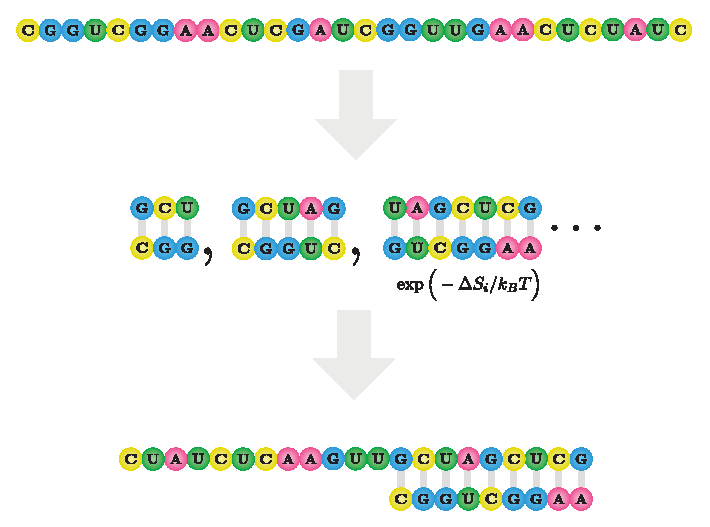
\includegraphics[scale = 1.1]{fig/rna_gillespie_algo}
\caption{Above is an illustration of our algorithm. We begin with a open strand sequence. From here we generate a move set of all possible moves, in this case, all the possible stems that could form. We assign a transition rate from the current state $S_{i}$ to the next state $S_{j}$. We then stochastically choose a move to happen from our probability distribution. We propogate our structure to this next move, then regenerate a move set with new transtion rates. We continue to do this until we have reached our maximum running time. The result is our folded structure. }
\label{fig:gill_algo}
\end{figure}

\begin{figure}[H]
\begin{small}
\begin{verbatim}
Sequence: CGGUCGGAACUCGAUCGGUUGAACUCUAUC
Time: 0.1945s | Added Stem: [[10, 17], [11, 16]] | Current Structure: ..........((....))............
Time: 4.4331s | Added Stem: [[5, 29], [6, 28]] | Current Structure: .....((...((....))..........))
Time: 4.9914s | Added Stem: [[7, 19], [8, 18]] | Current Structure: .....((((.((....))))........))
Time: 6.2564s | Added Stem: [[1, 24], [2, 23]] | Current Structure: .((..((((.((....))))...))...))
\end{verbatim}
\end{small}
\caption{A sample output from our algorithm.}
\end{figure}

\begin{multicols}{2}
\subsection{Results and Discussion}

In this section, we present and discuss the benchmark results of our stem level gillespie algoritm and compare them with benchmark results of Vienna RNA program \cite{Lorenz2011}. We tested our algorithm on the second dataset mentioned above, which was derived from the Rfam database. Recall this dataset consisted of approximately 30 variable length RNA sequences.

\begin{figure}[H]
\centering
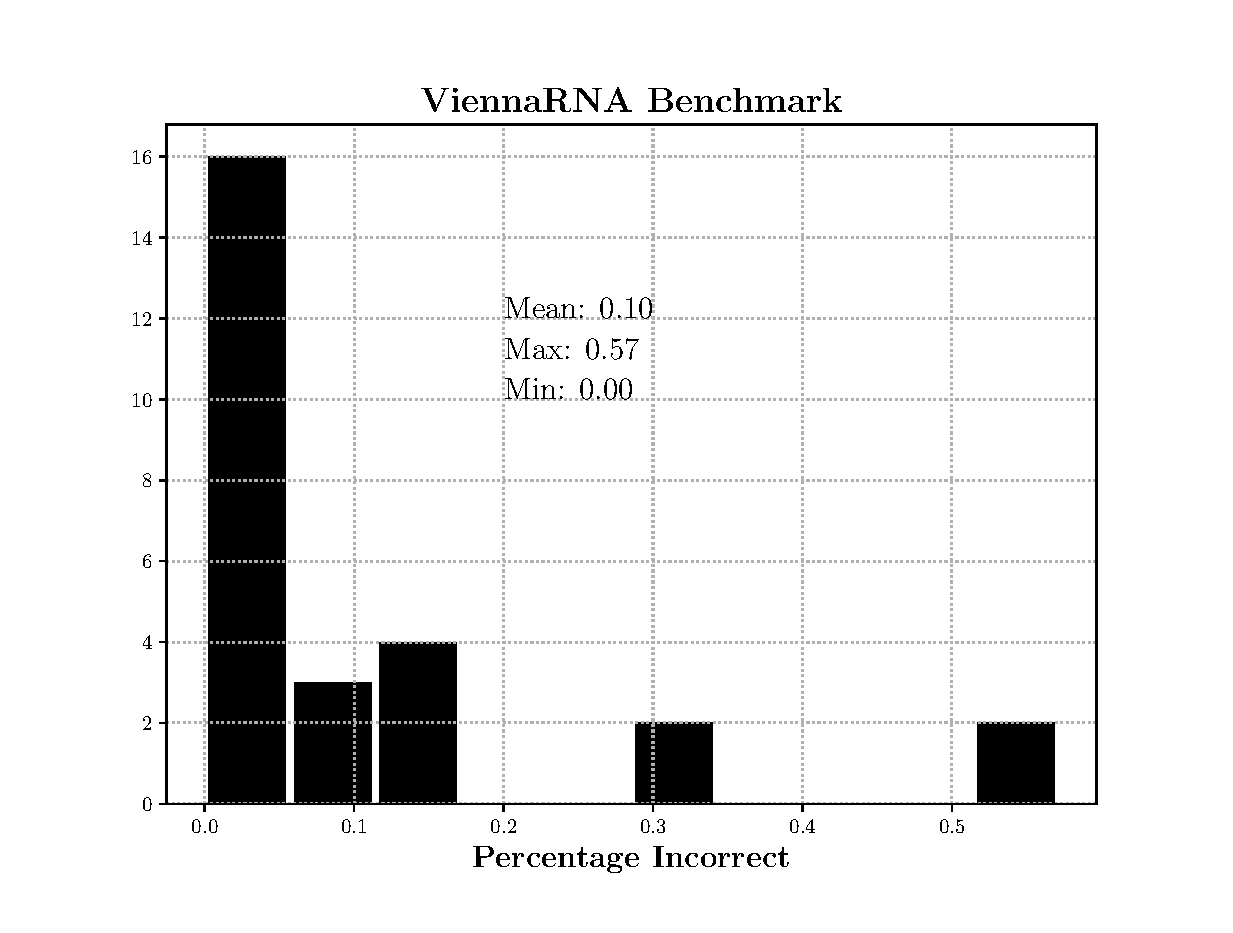
\includegraphics[width = 0.55\textwidth]{fig/v_rna_bench}
\caption{To benchmark our performance, we compared our algorithm to a popular RNA secondary structure predictor Vienna RNA \cite{Lorenz2011}. The $x$-axis is the percentage of the structure that we incorrectly predicted. The mean was $10\%$, the worst prediction was $0.57\%$, and the best prediction was $57\%$. }
\label{fig:vbench}
\end{figure}

In order to quantify the performance of our algorithm, we first obtain benchmark results on ViennaRNA's performance on our dataset. In Figure \ref{fig:vbench}, we have plotted a histogram of ViennRNA's performance. The histogram shows the percentage of the secondary structure that ViennaRNA predicted incorrectly. We can see that the average error was about $10\%$. The worst prediction was $57\%$ and the best prediction was $0\%$ or $100\%$ correct.

We now use the same data set with the Gillespie algorithm. Again, we have plotted a histogram of our program's performance. We can see from Figure \ref{fig:gill} that on average we predicted $38\%$ of the secondary structure incorrectly. Our best prediction was only $21\%$ incorrect and our worst prediction was $54\%$ incorrect.

\begin{figure}[H]
\centering
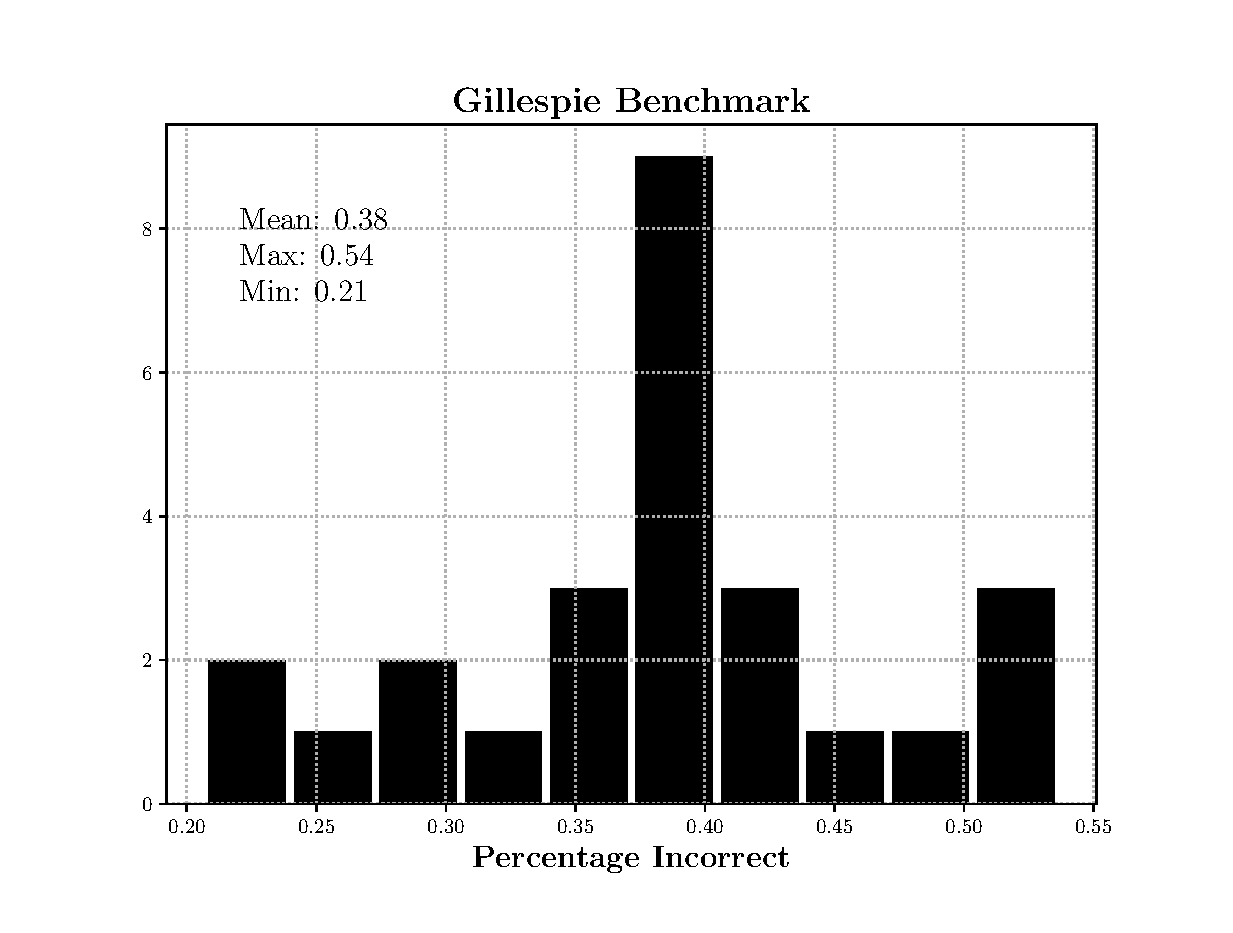
\includegraphics[width = 0.55\textwidth]{fig/gill_bench}
\caption{A histogram of the gillespie algorithm's performance. The $x$-axis represents the percentage of the structure that was incorrectly predicted by our algorithm. The mean is $38 \%$, the worst predction  was $54\%$, and the best prediction was $21 \%$.}
\label{fig:gill}
\end{figure}

Compared to ViennaRNA our stem level Gillespie algorithm was inferior in performance. However, we have one advantage that ViennaRNA does not. Our algorithm considers pseudoknotted structures. This gives a tremendous advantage when compared to 
\end{multicols}


\section{Conclusion}

\newpage
\nocite{*}
\printbibliography
\end{document}
